\section{Prediction Model}\label{prediction_model}
To learn from labelled patient dataset and be able to properly predict 
the occurence or not of Malaria given a new patient, we harness the logistic 
regression function as our \emph{classifier}. 
In this section, we briefy recall the basic of the logistic regression function
and how it can act as a binary classifier. We start by introducing the binary 
classification problem we have to solve in the study.

% binary classification problem for Malaria
\subsection{Binary classification problem}
Let us assume two given classes of Malaria diagnostic: \emph{Malaria} and \emph{Not-Malaria}.
We also consider \textsc{P} and \textsc{C} as respectively the set of patients and a prediction model.
A patient \emph{p} in \textsc{P} is defined by a set of pairs $(a_1, v_1), (a_2, v_2), \ldots, (a_n, v_n)$
where $a_i$ and $v_i$, for each $1\leq i\leq n$, respectively corresponds to a given Malaria feature and its associated value defined
as follows.
\begin{equation}
v_i = \left\{
\begin{array}{rl}
1 &\text{if $a_i$ is observed} \\
0 &\text{otherwise} \\
\end{array}
\right.
\end{equation}

\begin{definition}{(Our prediction problem)}
We define our binary classification problem for the prediction of the occurrence
or not of Malaria on a given patient dataset as a mapping \textsc{C} of every patient p in \textsc{P} 
to one and only one class in \{Malaria, Not-Malaria\}. Formally, we present such a mapping as \textsc{C}: \textsc{P} $\mapsto$ \{Malaria, Not-Malaria\}.
\end{definition}


We define and use  \textsc{C} with the help of the logistic regression for the specific purpose of our study. 
% Logistic regession function
\subsection{Logistic regression}
The logistic regression (a.k.a the logit function) is a statistical model used in the machine learning domain for binary classification \cite{Ch14}.
In its basic form, it is based on a logistic function to model a binary dependent variable \cite{Ho00,Sa14}.
As an input, the logistic regression  takes qualitative or/and ordinal predictive variables (e.g. the presence
or not of fever given a patient) in order to measure the probability of the outcome (e.g. the occurrence or not of the Malaria) 
by using the \emph{Sigmoid function}. Figure \ref{sigmoid_curve} shows the shape of the curve of the Sigmoid function. 

% The curve of the logistic regression
\begin{figure}[ht]
\centering
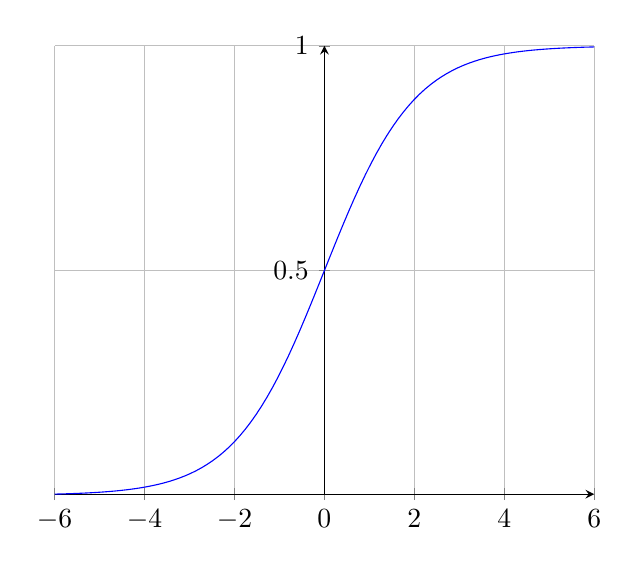
\begin{tikzpicture}
    \begin{axis}%
    [
        grid=major,     
        xmin=-6,
        xmax=6,
        axis x line=bottom,
        ytick={0,.5,1},
        ymax=1,
        axis y line=middle,
    ]
        \addplot%
        [
            blue,%
            mark=none,
            samples=100,
            domain=-6:6,
        ]
        (x,{1/(1+exp(-x))});
    \end{axis}
\end{tikzpicture}
\caption{The curve of the Sigmoid function}\label{sigmoid_curve}
\end{figure}

The logistic regression is one of the most used multi-valued models in epidemiology \cite{Am02,Pr05} (i.e. the study of the incidence,
 distribution, and possible control of diseases and other factors relating to health issues that can affect groups of population).
In such a context, the variable to explain is often the occurrence or not of an event like a disease and the explanatory 
variables, i.e. the features, are those that highly impact the occurrence of this event, i.e. variables assessing the exposure to a 
risk factor or a protective factor, or a variable representing the confusion factor.
The main interest of using logistic regression is its ability to quantify the strength of the relationship between each explicative 
variable and the variable to explain, given the other variables integrated to the model \cite{Am02}. 

% formal definition of the logistic model
\subsubsection{Formal definition  of our regression  model.}
Let us assume that \textsc{Y} represents the variable we are trying to explain in this study, i.e. the variable which models the occurrence or not of Malaria and whose 
two classes \emph{Malaria} and \emph{Not-Malaria} are respectively denoted by \textsc{M+} and \textsc{M-}. 

In the special case of only one explicative variable \emph{a} (which case corresponds to a simple regression), formally
the model is written as follows.

\begin{equation}
\textsc{Pr}(\textsc{M+} ~|~ \emph{a}) = \frac{e^{\alpha + \beta\times \emph{a} }}{1 + e^{\alpha + \beta\times \emph{a} }}
\label{simple_regression}
\end{equation}
where the coefficients $\alpha$ abd $\beta$ are the parameters of the model.

\textsc{Pr}(\textsc{M+} ~$|$~ \emph{a}) measures the probability of the occurrence of Malaria if the variable \emph{a} is observed.
Figure \ref{sigmoid_curve} represents the corresponding logistic function \emph{f(a)}. Again, the main interest of this function
lies in the simplicity of reaching an estimation of an odds ratio (OR) which measures the strength of the association between the 
disease \textsc{M} and an exposure variable in a regression analysis. Indeed if the value exposure variable is either $0$ (the variable is not observed)
or $1$ (the variable is observed) as in our setting, the model enables to obtain after some simplifications OR = $e^{\beta}$. The coefficient $\beta$ 
of the exposure variable in the logistic model is then the logarithmic of the odds ratio which measures the relationship between the explanatory variable 
(sign or symptom) and the disease (Malaria); this eases the analysis of the results of the logistic regression. 

An extension of the simple regression to a model with multiple variables (a.k.a multiple regression) is straightforward as we show with the formula below.

\begin{equation}
\textsc{Pr}(\textsc{M+} ~|~ \emph{$a_1$},\emph{$a_2$}, \ldots, \emph{$a_n$}) = \frac{e^{\alpha + \sum_{i=1}^{n} \beta_i \times \emph{$a_i$} }}{1 + e^{\alpha + \sum_{i=1}^{n} \beta_i \times \emph{$a_i$} }}
\label{multiple_regression}
\end{equation} 
where to every variable \emph{$a_i$} is associated a coefficient $\beta_i$. The corresponding odds ratio OR$_i$, quantifying the relationship between \emph{$a_i$} and \textsc{M+} is equal to $e^{\beta_i}$.

% Selection of the final model
\subsubsection{Selection of the final model.}  
